\subsection{Heat Maps}
This section will cover all the aspects of the heat maps use case.This use case is chosen as it is a vital part of the entire system.The data that is recorded will be used to create the heat maps that can then later be used to analyse the data and be used for future uses.

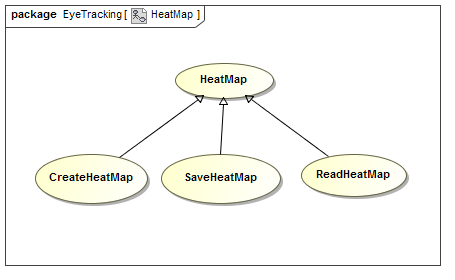
\includegraphics[scale=0.5]{Diagrams/Use_Case_Diagram__HeatMap.png}

The following sub use cases are included in this use case:
\subsubsection{CreateHeatMap}
This use case deals with the creation of the Heat map from the recorded data.The data is used to show where the user has viewed the media item the most.
\begin{itemize}
\item Pre-condition: Data must be already recorded.
\item Post-condition: Heat map of the data is created.
\item Request Data Structure: HeatMap.CreateHeatMap(Data[]).
\item Return data Structure: Heatmap is created
\end{itemize}
\subsubsection{ReadHeatMap}
This use case deals with the viewing of the Heat map from the recorded data.Once the heat map is created the users will be able to see the heat map and view the data.
\begin{itemize}
\item Pre-condition: Heat map must have been created.
\item Post-condition: Heat map of the data is viewable and can be further analysed.
\item Request Data Structure: HeatMap.ReadHeatMap(heatmapID).
\item Return Data Structure: Heat map is viewable.
\end{itemize}
\subsubsection{SaveHeatMap}
This use case deals with the saving of the Heat map from the recorded data.The heat map will be saved on the users computer to be viewed at a later date.This will save only the heat map.
\begin{itemize}
\item Pre-condition: Heat map must have been created.
\item Post-condition:Heat map of the data is saved.
\item Request Data Structure:HeatMap.SaveHeatMap(Data[]).
\item Return Data Structure:Heatmap is saved.
\end{itemize}
	
	
	
	\subsubsection{Save Heat Maps}
	The saving of the heat maps is important to the system as it will allow the users to save data of a whole array of data and then use and compare them on other applications.The heat map will serve as an overlay for the media type and be placed over the media.The saving of heat maps can be divided into three subsections, namely SaveOnImage,SaveOnVideo and SaveOn3DModel.
	\newline
		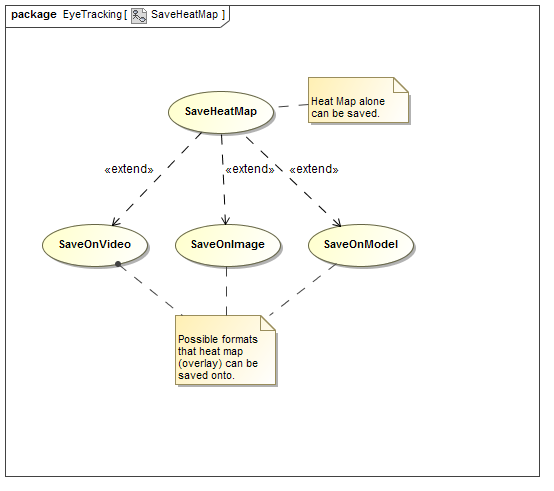
\includegraphics[scale=0.5]{Diagrams/Use_Case_Diagram__SaveHeatMap.png}
		\subsubsection{SaveOn2DModel}
The heat map that is created for a 2DModel media type will be saved and then applied to the 2DModel to see the heat map over the 2DModel to indicate where the user has viewed the most.
\begin{itemize}
\item Pre-condition: Heat map must have been created and the 2DModel of the heatmap must be available.
\item Post-condition: Heat map of the data is viewable on the 2DModel as an overlay.
\item Request Data Structure: HeatMap.SaveOn2DModel(heatmapID,2DModelID).
\item Return Data Structure: Heat map of the data is placed over the 2DModel.
\end{itemize}

		\subsubsection{SaveOnVideo}
The heat map that is created for a video media type will be saved and then applied to the video to see the heat map over the video to indicate where the user has viewed the most.The heat map will follow the video as the video plays and be changed as time passes.
\begin{itemize}
\item Pre-condition: Heat map must have been created and the video must be available.
\item Post-condition: Heat map of the data is viewable on the video as an overlay  and tracks the video position to be changed as the video plays.
\item Request Data Structure: HeatMap.SaveOnImage(heatmapID,ImageID).
\item Return Data Structure: Heat map of the data is placed over the video.
\end{itemize}

		\subsubsection{SaveOn3DModel}
The heat map that is created for a 3DModel media type will be saved and then applied to the 3DModel to see the heat map over the 3DModel to indicate where the user has viewed the most.The 3DModel can be either a 2D or 3DModel.
\begin{itemize}
\item Pre-condition: Heat map must have been created and the 3DModel of the heatmap must be available.
\item Post-condition: Heat map of the data is viewable on the 3DModel as an overlay.
\item Request Data Structure: HeatMap.SaveOn3DModel(heatmapID,3DModelID).
\item Return Data Structure: Heat map of the data is placed over the 3DModel.
\end{itemize}
		
\subsection{Models}
This section details all the different types of media or models that heat maps can be created for and saved onto.There are three types of models Video,2D and 3D.The heatmaps are created based on the models and their types.
\newline
	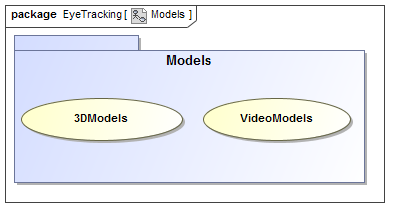
\includegraphics[scale=0.5]{Diagrams/Use_Case_Diagram__Models.png}
	
	
	\subsubsection{3D Models}
	3D Models will be taken into the system and then will be rendered and will be viewable to the user.The heatmap will then be allowed to be saved on the 3D model and then from there can be viewed with the heatmap as an overlay.
	\newline
		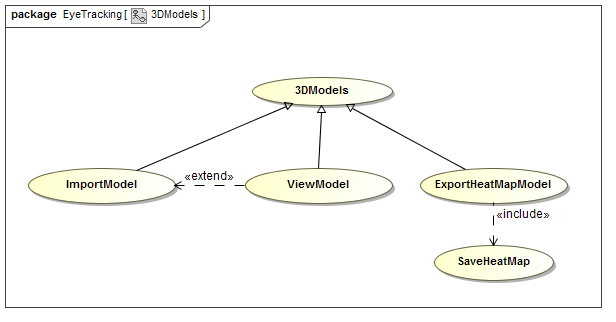
\includegraphics[scale=0.5]{Diagrams/Use_Case_Diagram__3DModels.png}
\begin{enumerate}
\item{ImportModel}
\newline
The heat map that is imported for a 3DModel media type will be saved in the system so that eye recording can be done on the media and that a heat map can be created for and be applied to it at a latter stage.
\begin{itemize}
\item Pre-condition: 3D model must exist.
\item Post-condition: Recording can be done on the model.
\item Request Data Structure: HeatMap.3DModeImport(3DModelID).
\item Return Data Structure: Rendered data model is imported.
\end{itemize}

\item{ViewModel}
Once the model is imported the users can view this and a recording of the eye can then be recorded for that specific model.
\begin{itemize}
\item Pre-condition: 3D model must have been imported .
\item Post-condition: 3D model is viewable and can be recorded on.
\item Request Data Structure: HeatMap.View3DModel(3DModelID).
\item Return Data Structure: Viewable 3D model
\end{itemize}

\item{ExportHeatMapModel}
The model will have had recording done to it and then a heat map will be applied to the model.This can then be exported so that it can be viewed at a letter date. 
\begin{itemize}
\item Pre-condition: Heat Map must be created and Model Imported.
\item Post-condition: Exported Model With heatmap on it to be viewed.
\item Request Data Structure: HeatMap.ExportHeatMap3DModel(heatmapID,3DModelID).
\item Return Data Structure: Model with heat map.
\end{itemize}

\end{enumerate}

	\subsubsection{2D Models}
	The 2D models can be imported into the system.The model will most often be a image of a jpeg file extension.The image can be imported and have recording done on it.The heat map is created and applied to it.
	\newline
		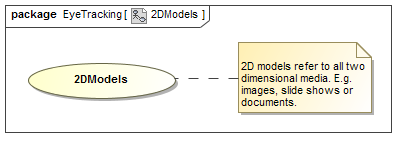
\includegraphics[scale=0.5]{Diagrams/Use_Case_Diagram__2DModels.png}
		
		\begin{enumerate}
\item{ImportModel}
\newline
The heat map that is imported for a 2DModel media type will be saved in the system so that eye recording can be done on the media and that a heat map can be created for and be applied to it at a later stage.
\begin{itemize}
\item Pre-condition: 2D model must exist,a image preferable.
\item Post-condition: Recording can be done on the model.
\item Request Data Structure: HeatMap.2DModeImport(2DModelID).
\item Return Data Structure: Rendered image is imported.
\end{itemize}

\item{ViewModel}
Once the model is imported the users can view this and a recording of the eye can then be recorded for that specific model.
\begin{itemize}
\item Pre-condition: 2D model(image) must have been imported .
\item Post-condition: Image is viewable and can be recorded on.
\item Request Data Structure: HeatMap.View2DModel(2DModelID).
\item Return Data Structure: Viewable image
\end{itemize}

\item{ExportHeatMapModel}
The image will have had recording done to it and then a heat map will be applied to the image or 2D model.This can then be exported so that it can be viewed at a later date and have a heat map placed on it. 
\begin{itemize}
\item Pre-condition: Heat Map must be created and Model Imported.
\item Post-condition: Exported Model With heatmap on it to be viewed.
\item Request Data Structure: HeatMap.Export2Dmodel(2DModelID).
\item Return Data Structure: Model with heat map.
\end{itemize}

\end{enumerate}
		
		
	\subsubsection{Video Models}
	A video can be easily imported into the system.The video can have recording done onto it and data stored.The data can then be used to create a heatmap that is then applied to the video second by second.
	\newline
		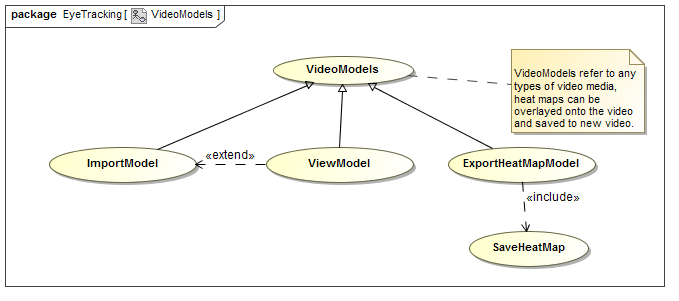
\includegraphics[scale=0.5]{Diagrams/Use_Case_Diagram__VideoModels.png}
		
		\begin{enumerate}
\item{ImportModel}
\newline
The heat map that is imported for a video media type will be saved in the system so that eye recording can be done on the media and that a heat map can be created for and be applied to it at a later stage.The heatmap will follow the video.
\begin{itemize}
\item Pre-condition: video must exist.
\item Post-condition: Recording can be done on the video.
\item Request Data Structure: HeatMap.VideoImport(videoID).
\item Return Data Structure: Rendered video is imported.
\end{itemize}

\item{ViewModel}
Once the video is imported the users can view this and a recording of the eye can then be recorded for that specific video.The heat map can be created and applied.
\begin{itemize}
\item Pre-condition: Video must have been imported .
\item Post-condition: Video is viewable and can be recorded on.
\item Request Data Structure: HeatMap.ViewVideo(videoID).
\item Return Data Structure: Viewable video.
\end{itemize}

\item{ExportHeatMapModel}
The video will have had recording done to it and then a heat map will be applied to the model.This can then be exported so that it can be viewed at a later date. The exported video will have a heat map on it.
\begin{itemize}
\item Pre-condition: Heat Map must be created and video Imported.
\item Post-condition: Exported video With heat map on it to be viewed.
\item Request Data Structure: HeatMap.SaveOnvideo(videolID).
\item Return Data Structure: Video with heat map.
\end{itemize}

\end{enumerate}
		
		
\subsection{Raw Information}
When recording happens on the system the raw information is saved.The raw information is important as it forms the basis for creating heat maps for specific.The raw information is saved on the system.The raw information can then be read as the raw data or put into a statistical formats.
\newline
	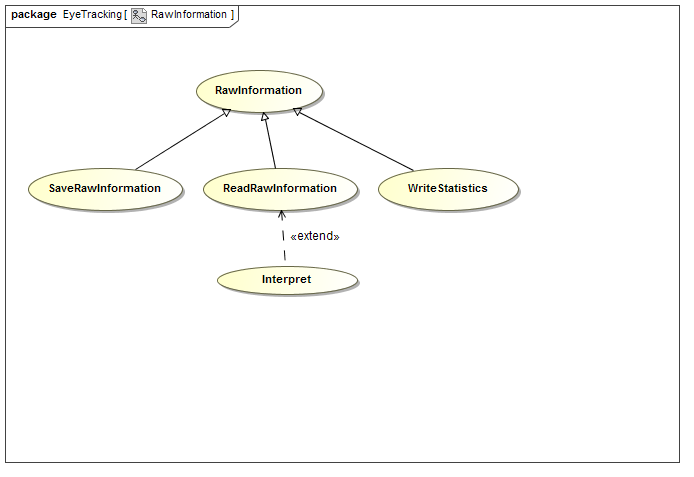
\includegraphics[scale=0.5]{Diagrams/Use_Case_Diagram__RawInformation.png}
	\subsubsection{SaveRawInformation}
When recording is done on the media the raw information will need to be saved so that it can be used at a later stage.This raw information is only temporarily saved and not saved for the life time of the media it is saved on.
\begin{itemize}
\item Pre-condition: Recording on a media type must have happened.
\item Post-condition: Data is saved and can be used later.
\item Request Data Structure: HeatMap.SaveRawInformation(data[]).
\item Return Data Structure: Raw array of data points saved.
\end{itemize}

	\subsubsection{ReadRawInformation}
Data can be read from a previously saved file.this will allow the user to import the data and then use it to compare to other data files.
\begin{itemize}
\item Pre-condition: Recorded data must be saved in a file.
\item Post-condition: Data is displayed.
\item Request Data Structure: HeatMap.ReadRawInformation(file).
\item Return Data Structure: data array with all data points.
\end{itemize}

	\subsubsection{WriteStatistics}
The writing of statistics is part of the Statistics uscase and all information can be found there regarding the sub use case
	
	
\subsection{Statistics}
Statistics on all the data is collected and will then be used to make a statistical page that can be analysed and then it can be easily compared at any time.
	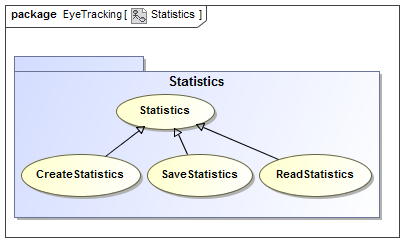
\includegraphics[scale=0.5]{Diagrams/Use_Case_Diagram__Statistics.png}
	
		\subsubsection{WriteStatistics}
Using the recorded data we can create a statistical analysis that can be viewed and used to compared data.
\begin{itemize}
\item Pre-condition: Recorded data must exist.
\item Post-condition: Data is turned into statistical data.
\item Request Data Structure: Stats.WriteStats(data[]).
\item Return Data Structure: Statistics in arrays.
\end{itemize}

		\subsubsection{SaveStatistics}
The statistics can be saved into a file so that they can be printed out and can be used as a hard copy.This will take all data and put it in a pdf or csv file.
\begin{itemize}
\item Pre-condition: Statistical data must exist.
\item Post-condition: Data is put into a report.
\item Request Data Structure: Stats.SaveStats(statsdata[]).
\item Return Data Structure: Save report in pdf or csv format.
\end{itemize}
	
	
\subsection{Record Eyes}
The recording of the eyes will be done using the camera.The data recorded will allow heat maps to be created.The heat maps can then be turned into overlays for the media types.the recording eyes use case uses a lot of sub use cases from other use cases such as SaveRawInformation.The recording of the information is important as this is used throughout.
\newline 
	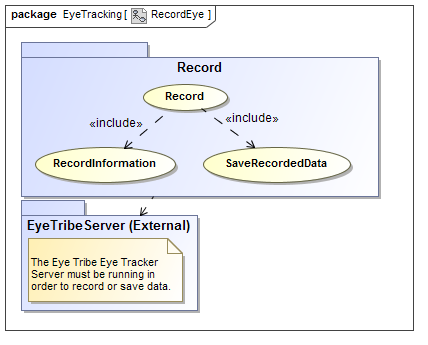
\includegraphics[scale=0.5]{Diagrams/Use_Case_Diagram__RecordEye.png}
	
\subsubsection{RecordInformation}
The information recorded will be sent to the OGAMA module to then be procesed and then this can be used to carry out functions in the system.
The
\begin{itemize}
\item Pre-condition: User needs to look at the media.
\item Post-condition: Data is recorded about the eye movements.
\item Request Data Structure: Recorder.Record(type).
\item Return Data Structure: Raw data in x,y and z co ordinates.
\end{itemize}



